% Chapter 4

\chapter{实验结果}
\section{性能评价}
本节利用Software-artifacts Infrastructure Repository (SIR)测试基准中提供的C/C++程序,对追踪过程的开销和解码过程的效率进行了评价。对于追踪阶段的开销,本实验比较了利用gcov进行的软件Profiling和利用Inel PT进行的硬件Profiling对程序执行造成的额外开销,包括编译后的可执行文件大小和程序运行的时间;对于解码过程,实验比较了设置不同的线程级数后对Intel PT追踪数据进行解码所耗费的时间。

实验过程中,配置了Intel PT追踪指定程序在每一个CPU上的全部运行,对每个CPU分配512KB的内存空间用于记录边带信息,分配4MB的空间用于记录Intel PT追踪数据,选取了SIR中的10个C/C++程序,通过gcc/g++在优化选项为-O2下编译,完成运行时的追踪和运行后的解码。实验运行环境为ubuntu18.04操作系统,Linux 5.3内核版本,Intel(R) Core(TM) i7-6700HQ CPU @ 2.60GHz 8核处理器,gcc-7.5.0编译器。

\begin{table}[ht]
  \centering
  \caption{源程序信息}
  \label{tab:7}
  \begin{tabular}{c|c|c|c|c|c|p{3cm}}
    \hline
    名称& 版本& 代码行& 函数/类& 测试用例& 语言& 描述\\ \hline
    flex& 1.1& 10459& 162& 525& C& 生成词法分析器\\ \hline
    grep& 1.2& 10068& 146& 470& C& 查找字符串\\ \hline
    gzip& 1.5& 5680& 104& 214& C& 压缩文件\\ \hline
    printtokens& 2.0& 726& 18& 4130& C& 词法分析\\ \hline
    printtokens2& 2.0& 570& 19& 4115& C& 词法分析\\ \hline
    schedule& 2.0& 412& 18& 2650& C& 优先级调度\\ \hline
    schedule2& 2.0& 374& 16& 2710& C& 优先级调度\\ \hline
    totinfo& 2.0& 565& 7& 1052& C& 信息统计\\ \hline
    vim& 1.0& 122169& 1999& 975& C& 编辑器\\ \hline
    concordance& 1.0& 1034& 5& 372& C++& 文本分析\\ \hline   
  \end{tabular}
\end{table}

实验中选择了SIR的10个C/C++程序,这些程序均是用于解决实际问题的真实程序,表\ref{tab:7}给出了选取的10个程序信息的描述,包括这些程序的名称、版本数、代码行、C程序的函数数量或C++程序的类数量、测试用例数、语言以及对程序的简单描述。每一个程序的测试选择都涵盖了SIR所提供的对应版本的全部测试用例,这些测试用例能够很好的覆盖到该程序的全部代码。在实验过程中,对每个程序的追踪与解码是对程序的全部测试用例进行的,以减少单个测试用例运行的偶然性。

\begin{table}[ht]
  \centering
  \caption{可执行文件大小和开销}
  \label{tab:8}
  \begin{tabular}{c|c|c|c}
    \hline
    程序名称& 普通编译& gcov选项编译& gcov选项开销\\ \hline
    flex& 229.0KB& 315.5KB& 37.8\%\\ \hline
    grep& 100.4KB& 180.6KB& 79.8\%\\ \hline
    gzip& 200.5KB& 260.7KB& 30.0\%\\ \hline
    printtokens& 16.8KB& 38KB& 126.1\%\\ \hline
    printtokens2& 13.6KB& 39.4KB& 190.0\%\\ \hline
    schedule& 13.5KB& 35.1KB& 160.0\%\\ \hline
    schedule2& 13.5KB& 34.7KB& 157.0\%\\ \hline
    totinfo& 13.3KB& 33.2KB& 149.6\%\\ \hline
    vim& 762.4KB& 1.3MB& 70.5\%\\ \hline
    concordance& 38.9KB & 67.0KB& 72.2\%\\ \hline
  \end{tabular}
\end{table}

\begin{table}[ht]
  \centering
  \caption{运行时间和开销}
  \label{tab:9}
  \begin{tabular}{c|c|c|c|c|c}
    \hline
    & 无Profiling& \multicolumn{2}{c|}{gcov}& \multicolumn{2}{c}{Intel PT}\\ \hline
    程序名称& 时间(s)& 时间(s)& 开销& 时间(s)& 开销\\ \hline
    flex& 1.000823& 1.188910&  18.6\%& 1.025578& 2.5\%\\ \hline
    grep& 1.112202& 1.219270&  9.6\%& 1.136327& 2.4\%\\ \hline
    gzip& 0.602457& 0.721433& 19.7\%& 0.613496& 1.1\%\\ \hline
    printtokens& 6.492572& 7.409447& 14.1\%& 6.684311& 2.9\%\\ \hline
    printtokens2& 6.270654& 6.973193& 11.2\%& 6.394291& 1.9\%\\ \hline
    schedule& 4.110148& 4.537002& 10.4\%& 4.155437& 1.1\%\\ \hline
    schedule2& 4.222819& 4.828388& 14.3\%& 4.294066& 1.6\%\\ \hline
    totinfo& 1.742980& 2.001803& 14.8\%& 1.757530& 0.8\%\\ \hline
    vim& 16.051291& 20.318301& 26.5\%& 16.546003& 3.1\%\\ \hline
    concordance& 4.390644& 4.787759& 9.0\%& 4.429473& 0.9\%\\ \hline
  \end{tabular}
\end{table}

\subsection{运行开销}
为了评价利用Intel PT硬件机制追踪运行时程序而对其造成的影响,实验中主要比较了基于软件的Profiling方式gcov和利用IntelPT进行硬件Profiling的开销,表\ref{tab:8}和表\ref{tab:9}给出了Profiling对程序运行过程开销对比。主要进行了两个方面的开销比较,首先表\ref{tab:8}给出了编译后源程序的大小,利用gcov进行软件层面的Profiling需要在编译时增加gcov相关编译选项,编译器在编译时向源程序进行插桩,注入额外的代码以收集运行时信息,从表\ref{tab:8}可以看出,这种机制会使可执行程序的大小发生明显的变化,平均会使可执行程序的大小增加64\%左右,而基于Intel PT的硬件Profiling借用硬件机制追踪,对源程序无侵入,因此并不会改变可执行程序的大小;表\ref{tab:9}给出了每个程序全部测试用例在无Profiling、利用gcov进行软件Profiling,利用Intel PT进行硬件Proiling的执行时间,图\ref{fig:cost}直观地给出了两种Profiling方式造成额外开销的对比,可以看出基于Intle PT的硬件Proiling方式造成的额外开销要远小于gcov软件Profiling造成的额外开销,最差情况下,gcov在vim中造成的额外开销甚至达到了26.5\%以上,而在vim中使用Intel PT进行的硬件Profiling造成的额外开销在其中仅有3.1\%,在本实验中,总体上,gcov造成的额外开销在10\%~30\%间,而Intel PT仅造成的额外开销小于5\%,远小于gcov造成的平均额外开销。
\begin{figure}[!htb]
  \centering
  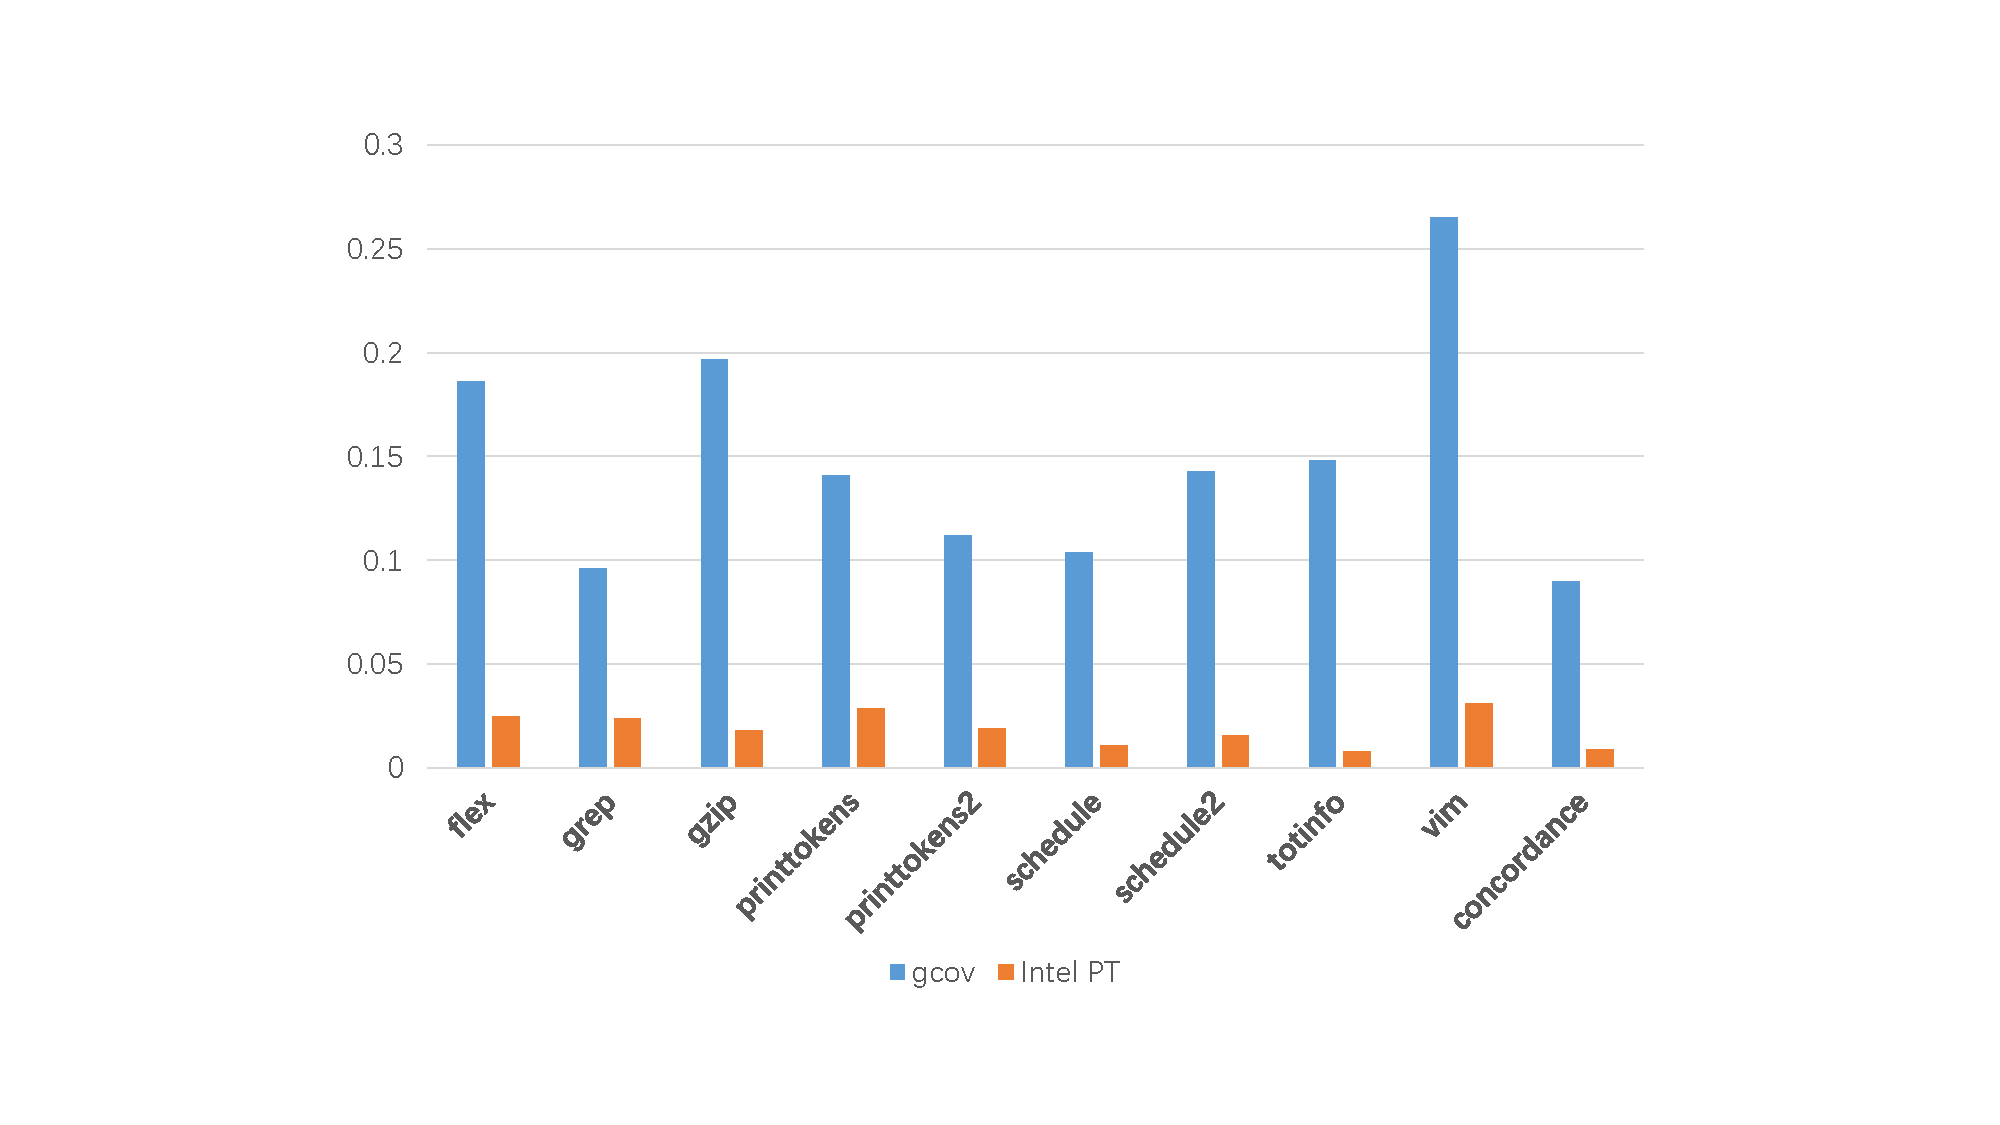
\includegraphics[width=1.0\textwidth]
  {figures/cost.pdf}\\
  \caption{运行开销}
  \label{fig:cost}
\end{figure}

\subsection{解码效率}
追踪程序的全部测试用例的执行并产生一系列追踪数据,这些追踪数据被导出到磁盘中,解码器对这些数据进行离线的解码重新构建程序的执行流。追踪过程中会产生大量的数据,表\ref{tab:10}和\ref{tab:11}给出了对每个程序的所有测试用例进行追踪导出的的总数据大小,对每个CPU的追踪数据包括记录的Intel PT数据和所需要的边带信息,Intel PT数据即Intel PT产生的一系列数据包,边带信息能够帮助我们了解程序执行时的内存和线程等信息,用于内存映像设置和执行线程信息获得等,对这些追踪数据进行解码需要耗费大量的时间,本课题通过实现解码阶段的并行化提高解码阶段的效率。

本节对实验中追踪SIR程序全部测试用例的Intel PT数据进行解码以评价实现的并行化解码器的性能。在对这些追踪数据进行解码时设置不同的并行级数(解码的线程数)进行比较,实验中首先测试非并行化的解码器(不进行Intel PT的数据划分,解码线程为1)的解码时间,然后将追踪数据划分为2-8份,并创建对应的解码线程进行并行解码。
\begin{table}[]
  \centering
  \caption{追踪数据大小(a)(单位:MB)}
  \label{tab:10}
  \begin{tabular}{c|c|c|c|c|c|c|c|c|c|c}
  \hline
        & \multicolumn{2}{c|}{flex} & \multicolumn{2}{c|}{grep} & \multicolumn{2}{c|}{gzip} & \multicolumn{2}{c|}{printtokens} & \multicolumn{2}{c}{printtokens2} \\ \hline
        CPU  & PT        & 边带      & PT        & 边带      & PT        & 边带      & PT            & 边带         & PT            & 边带          \\ \hline
  0 & 18.7      & 0.7           & 0         & 0.8           & 9.9       & 0.1           & 4.7           & 1                & 10.3          & 1.5               \\ \hline
  1 & 21.9      & 0.6           & 0         & 0.1           & 3.2       & 0.1           & 1.2           & 0.5              & 8.1           & 1.4               \\ \hline
  2 & 29.2      & 0.8           & 3.8       & 0.1           & 2.5       & 0.1           & 6.1           & 0.7              & 13.1          & 1.7               \\ \hline
  3 & 21.2      & 0.7           & 35.3      & 0.3           & 8.1       & 0.1           & 8.3           & 1.4              & 6.0           & 1.4               \\ \hline
  4 & 9.7       & 0.5           & 1.7       & 0.1           & 11.9      & 0.1           & 1.4           & 0.5              & 4.2           & 1.2               \\ \hline
  5 & 12.9      & 0.5           & 16.2      & 0.2           & 1.2       & 0.1           & 9.4           & 1.3              & 14.9          & 2.0               \\ \hline
  6 & 15.2      & 0.6           & 6.6       & 0.1           & 0.5       & 0.1           & 4.5           & 0.6              & 7.5           & 1.5               \\ \hline
  7 & 33.9      & 0.8           & 0         & 0.1           & 5.2       & 0.1           & 35.8          & 3.2              & 11.2          & 1.7               \\ \hline
  总和& \multicolumn{2}{c|}{168.2}& \multicolumn{2}{c|}{24.8}& \multicolumn{2}{c|}{43.4}& \multicolumn{2}{c|}{80.9}& \multicolumn{2}{c}{87.9}\\ \hline
  \end{tabular}
  \end{table}

  \begin{table}[]
    \centering
    \caption{追踪数据大小(b)(单位:MB)}
    \label{tab:11}
    \begin{tabular}{c|c|c|c|c|c|c|c|c|c|c}
    \hline
    &
    \multicolumn{2}{c|}{schedule} & \multicolumn{2}{c|}{schedule2} & \multicolumn{2}{c|}{totinfo} & \multicolumn{2}{c|}{vim} & \multicolumn{2}{c}{concordance}\\ \hline
    CPU      & PT          & 边带        & PT           & 边带        & PT        & 边带      & PT         & 边带        & PT        & 边带     \\ \hline
    0 & 10.1        & 1.0             & 0.4          & 0.8           & 0.6        & 0.1             & 50.1      & 3.6          & 37.4        & 0.9            \\ \hline
    1 & 18.9        & 1.6             & 0.3          & 0.1           & 2.4        & 0.2             & 67.3      & 4.1          & 46.1        & 1.2            \\ \hline
    2 & 1.3         & 0.2             & 19.2         & 0.1           & 5.6        & 0.2             & 79        & 4.5          & 51.2        & 1.1             \\ \hline
    3 & 6.5         & 0.8             & 12.1         & 0.3           & 1.6        & 0.2             & 70.2      & 4.5          & 31.5        & 0.8             \\ \hline
    4 & 6.5         & 0.8             & 14.9         & 0.1           & 7.7        & 0.4             & 74.8      & 4.0          & 43.8        & 0.7             \\ \hline
    5 & 1.0         & 0.3             & 6.6          & 0.2           & 9.1        & 0.6             & 66.1      & 4.2          & 27.9        & 0.8             \\ \hline
    6 & 7.3         & 0.8             & 0.2          & 0.1           & 4.5        & 0.3             & 63.5      & 4.1          & 43.8        & 0.9             \\ \hline
    7 & 2.7         & 0.6             & 7.7          & 0.1           & 1.5        & 0.1             & 69.4      & 4.4          & 41.8        & 0.9              \\ \hline
    总和& \multicolumn{2}{c|}{60.5}& \multicolumn{2}{c|}{67.3}& \multicolumn{2}{c|}{35.5}& \multicolumn{2}{c|}{574.0}& \multicolumn{2}{c}{373.3} \\ \hline 
    \end{tabular}
    \end{table}

\begin{table}[ht]
  \centering
  \caption{解码时间记录(单位:s)}
  \label{tab:12}
  \begin{tabular}{c|c|c|c|c|c|c|c|c}
    \hline
     & 1& 2& 3& 4& 5& 6& 7& 8\\ \hline  
    flex& 410.1& 224.0& 158.6& 127.4& 136.0& 121.2& 119.6& 110.5\\ \hline
    grep& 257.5& 160.0& 115.8& 94.8& 88.7& 85.7& 79.5& 77.6\\ \hline
    gzip& 384.5& 215.9& 157.1& 127.7& 126.1& 117.4& 109.8& 103.8\\ \hline
    printtokens& 199.8& 116.2& 84.4& 69.4& 71.8& 65.8& 65.2& 61.8\\ \hline
    printtokens2& 204.4& 116.9& 85.3& 71.5& 74.0& 68.6& 67.0& 62.2\\ \hline
    schedule& 148.5& 84.4& 59.9& 49.7& 50.5& 46.6& 46.7& 43.2\\ \hline
    schedule2& 163.8& 92.6& 66.7& 54.2& 55.8& 51.4& 50.6& 46.2\\ \hline
    totinfo& 94.9& 52.8& 38.4& 30.3& 32.3& 28.6& 27.4& 25.8\\ \hline
    vim& 1501.8& 898.4& 703.0& 620.7& 623.9& 590.2& 587.2& 578.1\\ \hline
    concordance& 799.8& 438.2& 314.4& 253.6& 265.9& 243.2& 233.6& 220.5\\ 
    \hline
  \end{tabular}
\end{table}

表\ref{tab:12}给出了全部实验的解码时间记录,包括非并行化解码以及设置并行级数为2~8时的解码时间,图~\ref{fig:decode-time1}和图~\ref{fig:decode-time2}直观地给出了非并行化解码器以及设置不同并行级数解码器的解码时间对照。可以发现,在该实验平台下,此并行化解码器最好情况下解码时间小于原来解码时间的1/3,表现最好的flex减少了非并行解码器73\%的解码时间,总体上,并行化解码器最好能够减少非并行解码器解码时间的61\%-73\%,且随着Intel PT追踪数据规模的增加,并行解码器对解码效率的提高依然较为明显,其中较大数据规模的concardance的解码时间仍然减少了非并行解码时间的70\%左右。



\begin{figure}[!htb]
  \centering
  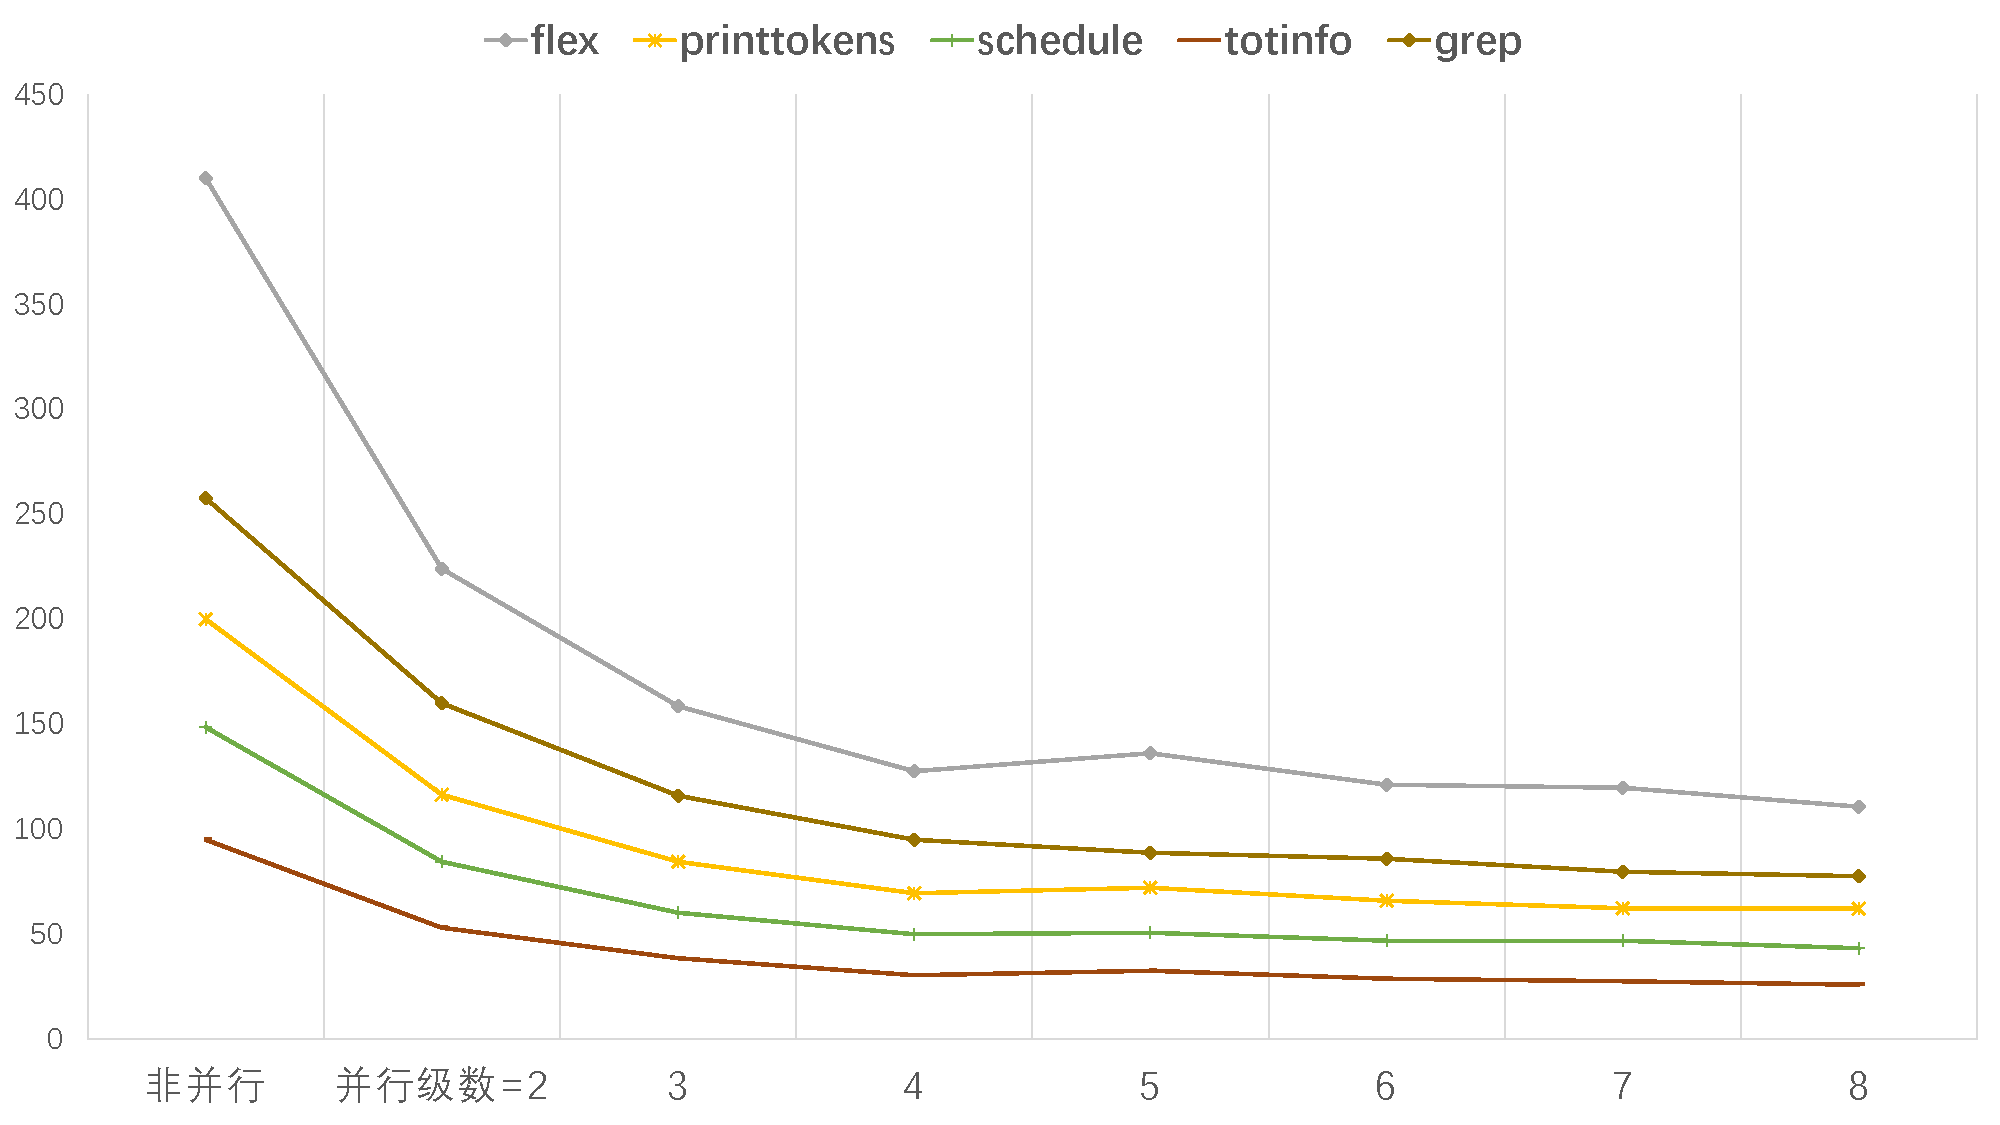
\includegraphics[width=0.8\textwidth]
  {figures/decode-time1.pdf}\\
  \caption{解码时间对照(a)}
  \label{fig:decode-time1}
\end{figure}

\begin{figure}[!htb]
  \centering
  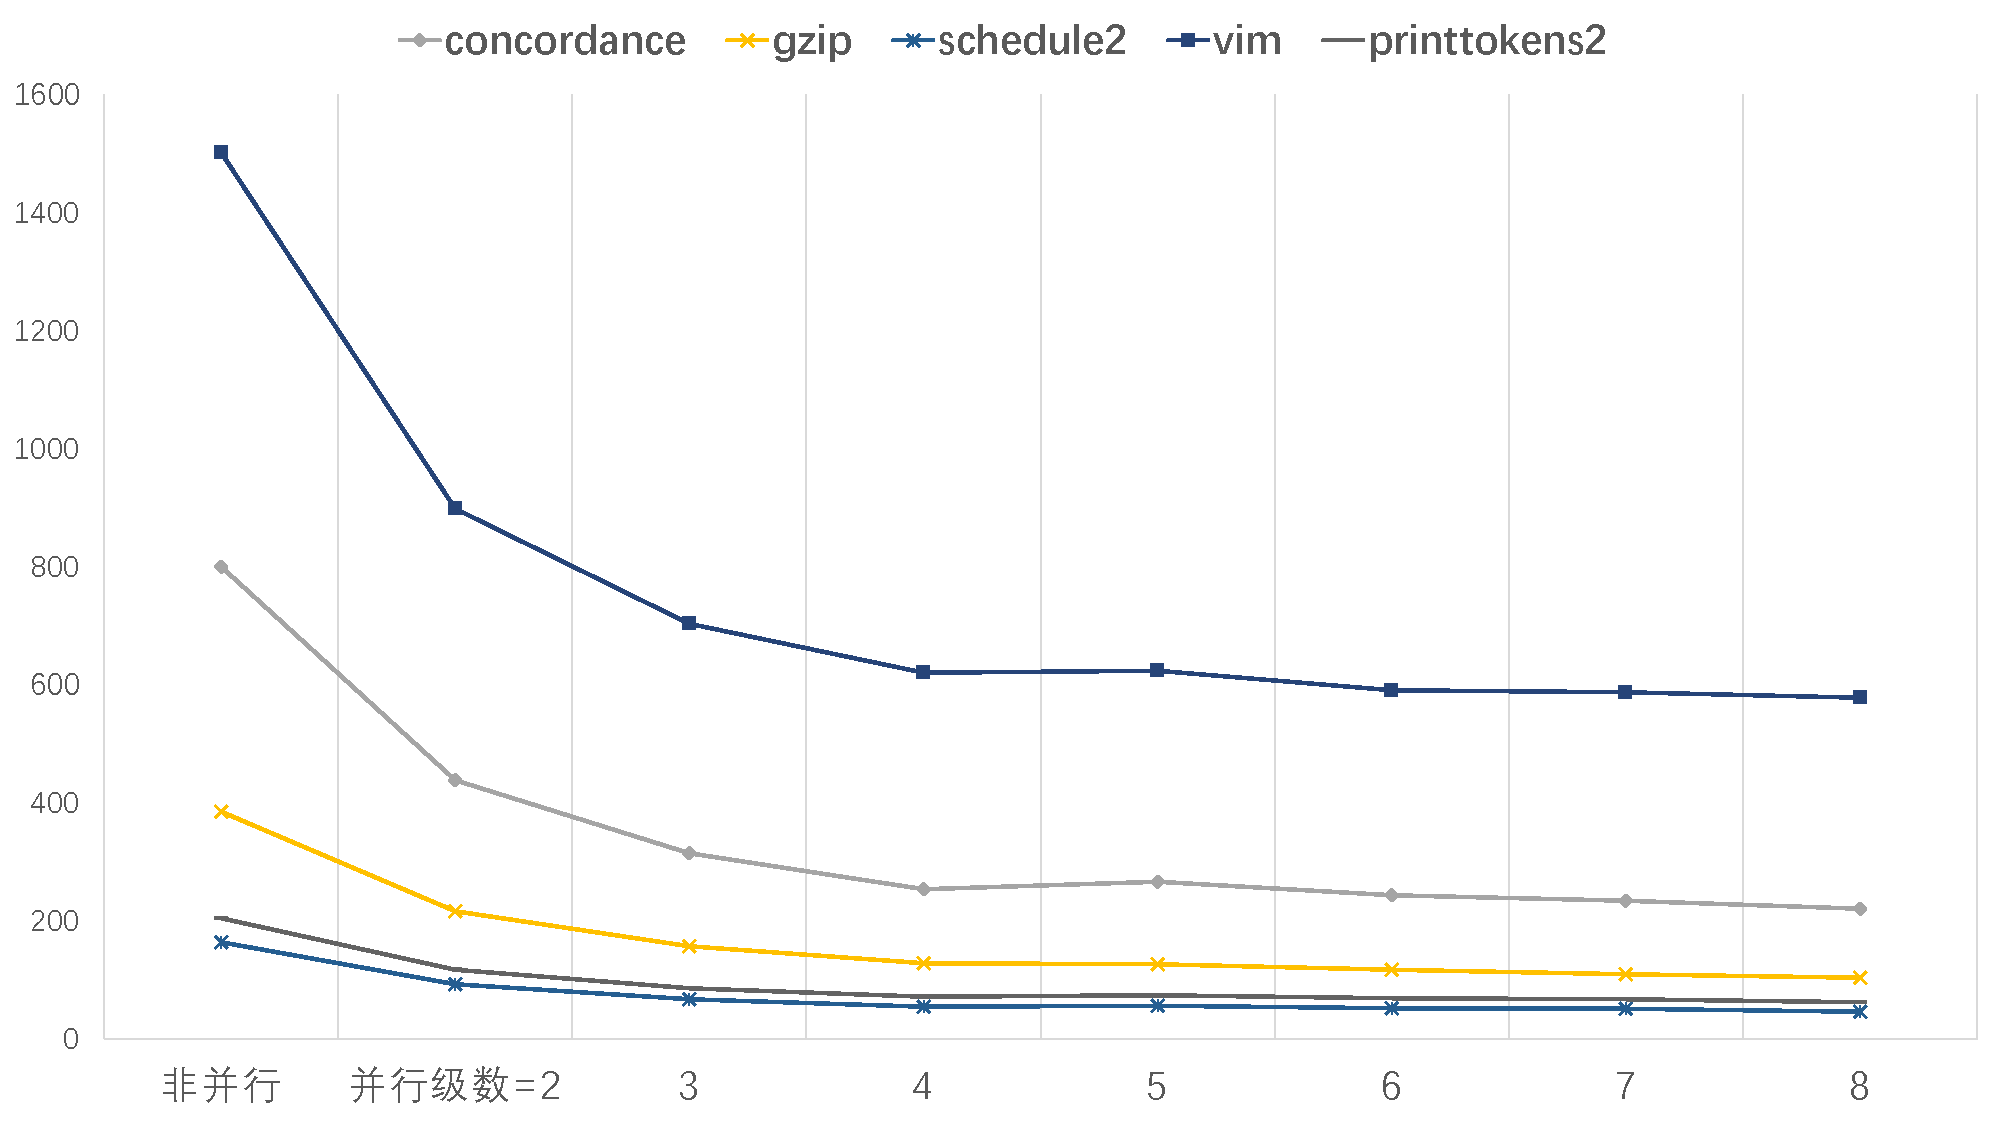
\includegraphics[width=0.8\textwidth]
  {figures/decode-time2.pdf}\\
  \caption{解码时间对照(b)}
  \label{fig:decode-time2}
\end{figure}



\section{源码Profiling结果}
此节给出了实现的C/C++程序Profiling工具的最终结果输出示例,如表\ref{tab:13}所示,表格左侧给出了源码信息,对于左侧所示的简单C程序,最终此Profiling工具能够给出类似于表\ref{tab:13}中间所示的函数调用层次关系,以及右侧所示的执行信息图,分别给出了源码所对应的每一个函数的调用次数以及每一行所对应的执行次数。
\begin{table}[ht]
\centering
\caption{源码级Profiling结果}
\label{tab:13}
\begin{tabular}{|l|p{3cm}|l|}
\hline
line 1 : \#include <stdio.h>& \dots& \dots\\
line 2 : &\quad main()& \dots \\
line 3 : int add(int a, int b)\{& \quad \quad add()& \dots/test.c\\
line 4 : \quad return a+b;&\quad \quad sub()& \quad div():  9801\\
line 5 : \}& \quad \quad mul()& \quad mul():  9801\\
line 6 :& \quad \quad div()& \quad sub():  9801\\
line 7 : int sub(int a, int b)\{& \quad \quad add()& \quad add():  9801\\
line 8 : \quad return a-b;& \quad \quad sub()& \quad main():  1\\
line 9 : \}& \quad \quad mul()& \quad \quad line:3		9801\\
line 10:& \quad \quad div()& \quad \quad line:4		9801\\
line 11: int mul(int a, int b)\{& \quad \quad add()& \quad \quad line:5		9801\\
line 12: \quad return a*b;& \quad \quad sub()& \quad \quad line:7		9801\\
line 13: \}& \quad \quad mul()& \quad \quad	line:8		9801\\
line 14: & \quad \quad div()& \quad \quad line:9		9801\\
line 15: int div(int a, int b)\{& \quad \quad add()& \quad \quad line:11		9801\\
line 16: \quad return a/b;& \quad \quad sub()& \quad \quad line:12		9801\\
line 17: \}& \quad\quad mul()& \quad \quad line:13		9801\\
line 18: & \quad \quad div() & \quad \quad line:15		9801\\
line 19: int main()\{& \quad \quad add() & \quad \quad line:16		9801\\
line 20: \quad int i, j;& \quad \quad sub()& \quad \quad line:17		9801\\
line 21: \quad for (i = 1; i < 100; i++)\{& \quad \quad mul()& \quad \quad line:19		1\\
line 22: \quad \quad for (j = 1; j < 100; j++)\{& \quad \quad div() & \quad \quad line:21		100\\
line 23: \quad \quad \quad add(i, j);& \quad \quad add()& \quad \quad line:22		9900\\
line 24: \quad \quad \quad sub(i, j);& \quad \quad sub() & \quad \quad line:23		9801\\
line 25: \quad \quad \quad mul(i, j);& \quad \quad mul() & \quad \quad line:24		9801\\
line 26: \quad \quad \quad div(i, j);& \quad \quad div() & \quad \quad line:25		9801\\
line 27: \quad \quad \}& \quad \quad add()& \quad \quad line:26		9801\\
line 28: \quad \}& \quad \quad sub() & \quad \quad line:29		1\\
line 29: \quad return 0;& \quad \quad mul()& \quad \quad line:30		1\\
line 30: \}& \dots & \dots \\
\hline
\end{tabular}
\end{table}

